\documentclass[11pt,a4paper]{article}
\usepackage[T1]{fontenc}
\usepackage{lmodern}
\usepackage{a4wide}
\usepackage[dvips]{graphicx}
\usepackage{float}

\usepackage[
pdfauthor={ACE Projekt Team},
pdftitle={Evaluation Algorithms},
pdfcreator={pdftex},
]{hyperref}

\usepackage{sectsty}
\allsectionsfont{\sffamily}

\usepackage{fancyheadings} 
\pagestyle{fancy} 
\lhead{\textsf{\textbf{ACE} \\ \small{a collaborative editor}}}
\chead{}
\rhead{
\parbox[c]{3cm}{
\includegraphics[height=0.875cm,width=3cm]{../../images/logo_BFH.eps}}
\parbox[c]{2.2cm}
{\tiny{\textsf{Berner Fachhochschule \\
Hochschule f�r \\
Technik und Informatik}}}}
\lfoot{}
\cfoot{\textsf{\thepage}}
\rfoot{}
\setlength{\headrulewidth}{0.6pt}
\setlength{\footrulewidth}{0.6pt}
\setlength{\topmargin}{-50pt}
\addtolength{\headheight}{50pt}

\usepackage{colortbl}

\newcommand{\headercol}[2]{\multicolumn{1}{|>{\bfseries\columncolor[gray]{0.82}}p{#1}|}{\textsf{#2}}}
\newcommand{\ace}[0]{\emph{ACE }}



\begin{document}
\setlength{\parindent}{0pt}

\newtheorem{defn}{Definition}

\bibliographystyle{plain}

\begin{titlepage}
\thispagestyle{empty}
  
\includegraphics[height=1.5in]{../images/pix.eps}

  \begin{center}

    {\fontsize{40}{45} \textbf{\textsf{ACE}}} \\
    \textsf{a collaborative editor} \\
        
    \vspace{36pt}
        
    {\huge{\textbf{\textsf{}}}} \\

    \vspace{36pt}

	\textsf{Berne University of Applied Sciences} \\
    \textsf{School of Engineering and Information Technology} \\
    
  \end{center}

  \vfill
  
  \begin{tabular}{ll}
   \hline

   \\

   \multicolumn{1}{>{\bfseries}p{1.5in}}{\textsf{Date:}} &
   \multicolumn{1}{>{}p{4.3in}}{\textsf{08.11.2005}}          \\
   
   \\
   
   \multicolumn{1}{>{\bfseries}p{1.5in}}{\textsf{Version:}}     &   
   \multicolumn{1}{>{}p{4.3in}}{\textsf{0.1}}                 \\

   \\
   
   \multicolumn{1}{>{\bfseries}p{1.5in}}{\textsf{Projectteam:}}                 &
   \multicolumn{1}{>{}p{4.3in}}{\textsf{Mark Bigler (biglm2@hta-bi.bfh.ch)}}  \\
   \multicolumn{1}{>{\bfseries}p{1.5in}}{}                                      &
   \multicolumn{1}{>{}p{4.3in}}{\textsf{Simon Raess (rasss@hta-bi.bfh.ch)}}    \\
   \multicolumn{1}{>{\bfseries}p{1.5in}}{}                                      &
   \multicolumn{1}{>{}p{4.3in}}{\textsf{Lukas Zbinden (zbinl@hta-bi.bfh.ch)}} \\   
   
   \\
   
   \multicolumn{1}{>{\bfseries}p{1.5in}}{\textsf{Receivers:}}                       &
   \multicolumn{1}{>{}p{4.3in}}{\textsf{Jean-Paul Dubois (doj@hta-bi.bfh.ch)}}       \\
   \multicolumn{1}{>{\bfseries}p{1.5in}}{}                                          &
   \multicolumn{1}{>{}p{4.3in}}{\textsf{Claude Fuhrer (frc@hta-bi.bfh.ch)}}       \\

   \\
   
   \multicolumn{1}{>{\bfseries}p{1.5in}}{\textsf{Location:}}               &   
   \multicolumn{1}{>{}p{4.3in}}{\textsf{Subversion Repository}} \\

   \\  
   
   \hline
  \end{tabular}

\end{titlepage}

\newpage

\tableofcontents
\newpage
\listoftables
\listoffigures
\newpage


\section*{Versionskontrolle}

\begin{table}[!h]
 \begin{tabular}{|l|l|l|l|}
  \hline
  \headercol{0.6in}{Version}         & 
  \headercol{0.8in}{Datum}           &
  \headercol{1.2in}{Verantwortlich}  & 
  \headercol{2.8in}{Bemerkungen}     \\
  \hline
  0.1         & 15.03.2005  & rasss           &  Erste Version \\
  \hline
  0.2         & 22.03.2005  & rasss zbinl     &  �berarbeitung \\
  \hline
  0.3         & 30.03.2005  & zbinl           &  Projektspezifisches Vorgehensmodell \\
  \hline
  0.4         & 30.03.2005  & rasss zbinl     &  �berarbeitung Punkte 2, 3 und 4 \\
  \hline
  0.5         & 05.04.2005  & zbinl           &  �berarbeitung Appendix A.1 \\
  \hline
  0.6         & 06.04.2005  & zbinl           &  Anpassungen Punkte 2, 3 und 4 \\
  \hline
  0.7         & 06.04.2005  & Projektteam     &  Review \\
  \hline
  0.8         & 13.04.2005  & Projektteam     &  Letzte Anpassungen \\
  \hline
  1.0         & 13.04.2005  & Projektteam     &  Freigabe \\
  \hline
 \end{tabular}
 \caption{Versionskontrolle}
 \label{Versionskontrolle}
\end{table}

\begin{table}[!h]
 \begin{tabular}{|l|l|l|l|l|}
  \hline
  \headercol{0.9in}{}            & 
  \headercol{0.9in}{Stelle}      & 
  \headercol{0.8in}{Datum}       & 
  \headercol{0.6in}{Visum}       & 
  \headercol{2.0in}{Bemerkungen} \\
  \hline
  \textbf{Freigegeben}   & Projektteam &       &       &             \\
  \hline
  \textbf{Genehmigt}     &             &       &       &             \\
  \hline
 \end{tabular}
 \caption{Pr�fung/Genehmigung}
 \label{Pr�fung/Genehmigung}
\end{table}

\newpage


\section{Introduction}
The purpose of this report is to show usability requirements a user-friendly collaborative editor must have. The most usefull functions will be discussed in the following chapters. There existing also prototypes for some of these functions to ensure the realizability with JAVA text components.

\section{Usability}
Basicaly each user must be distinguishable from all the other users. To do that with different colors is probably one of the best solution. For example the red user has a dark red colored cursor, a light red color to highlight the text he changed and a red border around the text he selected. The users are listed with their colors in a separate window, so all participants can quite easy see which part in the multi-colored document belongs to which user. See \cite{usability} for more information about usability in groupware systems.

\subsection{Main View}
The main view is the users workspace where he can change the document or observe the other users. Important is to keep the main view as simple as possible. This means that it should not be overloaded with a lot of buttons, status labels, etc. because new users will loose their orientation.
\begin{figure}[H]
\centering
\frame{

\includegraphics[height=3cm,width=5cm]{../../images/gui/gui_main_view.eps}
}
\caption{Main View}
\end{figure}

\subsection{Multiple Cursors and Telepointers}
To display the cursors of the other participants is a very usefull feature for observing their changes. This additional cursors must be clearly distinguishable and assigned to a user. Coloring all cursors with the user color (e.g. the green users cursor is painted in dark green) will be the most comfortable way to realize that. Moreover, this cursors should have another form than the standard cursor.

As described above for multiple cursors, it will be user friendly to display the content of the document in different colors too. On this way all participants knows which part is from which user.
\begin{figure}[H]
\centering
\frame{
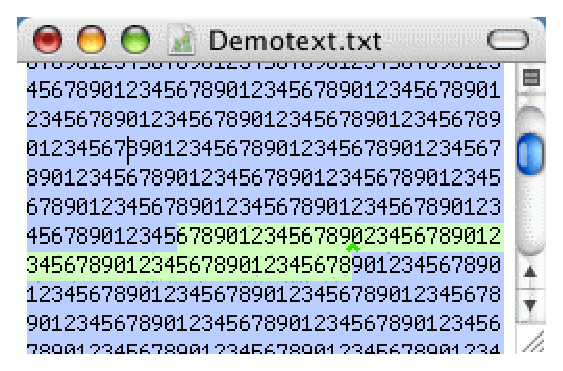
\includegraphics[height=3cm,width=5cm]{../../images/gui/gui_hlight_and_cursor.eps}
}
\caption{Multiple Cursors and Highlighted Text}
\end{figure}
The other users mouse cursors are called telepointers. With this telepointers it is possible to show or explain something in the document. It should be possible to activate/deactivate this telepointers because a lot of different cursors and telepointers can be confusing to the users.
\begin{figure}[H]
\centering
\frame{
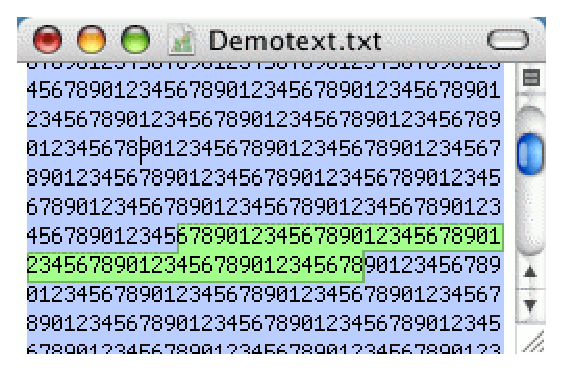
\includegraphics[height=3cm,width=5cm]{../../images/gui/gui_selection.eps}
}
\caption{Text-selection}
\label{Text-selection}
\end{figure}
The picture \ref{Text-selection} shows a possibility to represent selected text of another participant (in this case from the participant associated with the green color).

\subsection{Multi-user Scrollbar}
The aim of multi-user scrollbars is to give a coarse overview of all cursor positions in the document. A user will see his own position by a normal scrollbar and in addition a little colored symbol for the position of each other user.
\begin{figure}[H]
\centering
\frame{
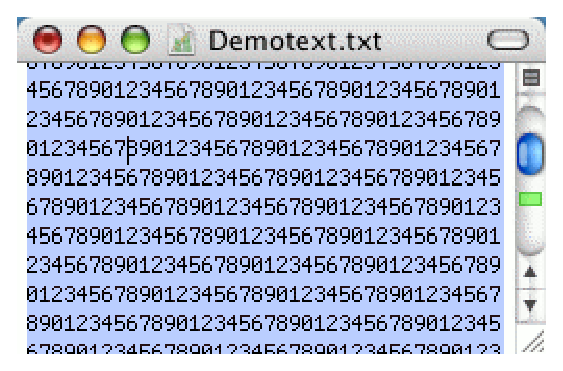
\includegraphics[height=3cm,width=5cm]{../../images/gui/gui_scrollbar.eps}
}
\caption{Multi-user Scrollbar}
\end{figure}

\subsection{Teleport and Split View}
- teleport -> easy showing with shortcut

- splitview -> permanent splitscreen

\subsection{Document and User Handling}
- share documents

- browser shared documents

- invite user / join document

- security and access management


\section{Prototypes}
\subsection{CustomPaint}
\paragraph{Purpose:}
\paragraph{Description:}
\paragraph{Notes:}

\subsection{CustomView}
\paragraph{Purpose:}
\paragraph{Description:}
\paragraph{Notes:}

\subsection{CustomDocument}
\paragraph{Purpose:}
- catch keyborad inputs
\paragraph{Description:}
\paragraph{Notes:}



\section{Other}
\subsection{Undo / Redo}
TODO: describe undo / redo

\subsection{Global Textcomponent Interface}
TODO: describe global interface

\subsection{Distribute Document Changes}
TODO: describe doc changes



\newpage
\appendix

\section{Undo in multiuser collaborative applications}
\label{sect:undo}

The availability of undo in a multiuser collaborative application is valuable because features available in single-user applications should also be available in corresponding multi-user applications. However, supporting undo in a multiuser collaborative application is much more difficult than supporting undo in single-user interactive applications because of the interleaving of operations performed by multiple users in a collaborative computing environment.


\subsection{An Example}

To illustrate the difficulties, let us consider a collaborative editing session with two users and a shared text document containing the string '"abc'". Suppose user 1 issues the operation $O_{1} = Ins[2,X]$ to insert the character '"X'" at position 2 after the character '"a'". The resulting document state is '"aXbc'". After this, user 2 issues operation $O_{2} = Ins[2,Y]$ to insert character '"Y'" after the character '"a'" to get the resulting document state '"aYXbc'". Suppose user 1 wants to undo his last operation, i.e. $O_{1}$. Her intended effect is to remove the '"X'" thus resulting in a document state '"aYbc'". First, blindly picking the \emph{globally} last operation, i.e. $O_{2}$ will undo the wrong operation. Second, simply executing the inverse operation $\overline{O_{1}} = Del[2,X]$ to delete the '"X'" at position 2 in the current document state '"aYXbc'" will delete '"Y'" instead of '"X'".

This means that any group undo solution must meet the challenge of undoing operations in a nonlinear way and must be able to achieve the correct undo effect in a document state that has been changed by other users'' operations. It can be clearly seen that undo in a groupware system is highly related to operational transformations.


\subsection{Types of Undo}

Generally a user expects an undo to reverse their own last operation (\emph{local} undo) rather than the globally last operation (\emph{global} undo). So an undo framework for groupware systems needs to allow selection of an operation to undo based on who performed it. Undoing the globally last action can be problematic as just before one user presses undo, another user may issue an operation. The effect of the operation may get executed at the first users site just before he effectively invokes the undo action. This would not result in the undoing of an operation which the first user intended to undo.

Further an undo mechanism may be classified by whether it allows to undo an arbitrary operation (called \emph{selective} undo) or it is restricted to the \emph{chronological} order.

It is still an open question how to select operations to be undone in a selective undo system. To undo the chronoligically last operation of the local user, the single familiar undo menu or shortcut is sufficient as it is always clear wich operation has to be undone.


\subsection{Existing Undo Solutions}

\subsubsection{DistEdit System}
The DistEdit system \cite{prakash94} allows operations to be undone in any order. However, it may be that an operation is not undoable because it conflicts with a later executed operations. The conflicts occur if a later operation happens at the same index as the operation to undo. They managed to solve some conflicting situations, but still a few remained in the finished system.

\subsubsection{adOPTed undo}
In the \emph{adOPTed} algorithm (see \ref{algo:adopted}) undo is supported by operational transformation. It allows to undo the chronological last operation of a user (it is implemented only for the local user but would it would be possible to extend it to an arbitrary user). To undo an operation, an inverse of this operation is generated by a special \emph{mirror} operator. This inverse operation must be placed at a valid location in the corresponding dimension of the interaction graph. No conflict can occur in undoing any operation. Another special operator called \emph{folding} is used for a correct working system. See \cite{ressel99} for a detailed description of this undo system.

\subsubsection{GOTO undo}
Sun \cite{sun02b} described an undo mechanism for the \emph{REDUCE} prototype. It is using the \emph{GOTO} algorithm (see \ref{algo:goto}) for \emph{do} and an algorithm called \emph{ANYUNDO} for \emph{undo}. The algorithm allows undoing arbitrary operations, so it is a selective undo system. The algorithm is described in great detail along many possible problems and how they were solved in this algorithm.



\section{Vector Time}
\label{sect:vectortime}

Most algorithms use \emph{vector time} to determine causal relations. Each site maintains a state vector $v$ that has $n$ components. $n$ is the number of participating sites. $S$ is the local site. The $i$-th component of $v$ denoted as $v[i]$ represents the number of operations executed from site $i$ at site $S$ (the local site). 

\begin{defn}
  For two time vectors u, v \\
  $u \leq v$ iff $\forall i : u[i] \leq v[i]$ \\
  $u < v$ iff $u \leq v$ and $u \not= v$ \\
  $u \parallel v$ iff $\neg(u < v)$ and $\neg(v < u)$
\end{defn}

Notice that $\leq$ and $<$ are partial orders. The \emph{concurrency relation} $\parallel$ is reflexive and symmetric.

The above definition gives us a very simple method to decide whether two events $e$ and $e'$ are causally related or not: We take their timestamps (vector times) and check whether $C(e) < C(e')$ or $C(e') < C(e)$ where $C(x)$ determines the timestamp of $x$. If the test succeeds, the events are causally related. Otherwise they are independent.




\newpage
\bibliography{ace}

\end{document}
